\documentclass[tikz,border=20pt]{standalone}
\usetikzlibrary{arrows.meta}
\usepackage{tikz}


\definecolor{red}{HTML}{D44D13}
\definecolor{green}{HTML}{77C114}
\definecolor{blue}{HTML}{045275}

\definecolor{viridisYellow}{HTML}{FDE725}


\definecolor{viridisCyan}{HTML}{404387}
\definecolor{viridisGreen}{HTML}{29788E}
\definecolor{viridisTeal}{HTML}{22A784}
\definecolor{viridisLime}{HTML}{7AD151}
\definecolor{viridisYellowLight}{HTML}{FDE725}

\definecolor{mygreen}{HTML}{77C114}

\def\AYA{\footnotesize{\texttt{AYA}}}
\def\EDGE{\footnotesize{\texttt{REL}}}
\def\Care{\footnotesize{\texttt{CARE}}}

\def\within_color{gray}

\begin{document}

% \begin{wrapfigure}{l}{0.5\textwidth} % 'r' for right, 'l' for left
%     \centering

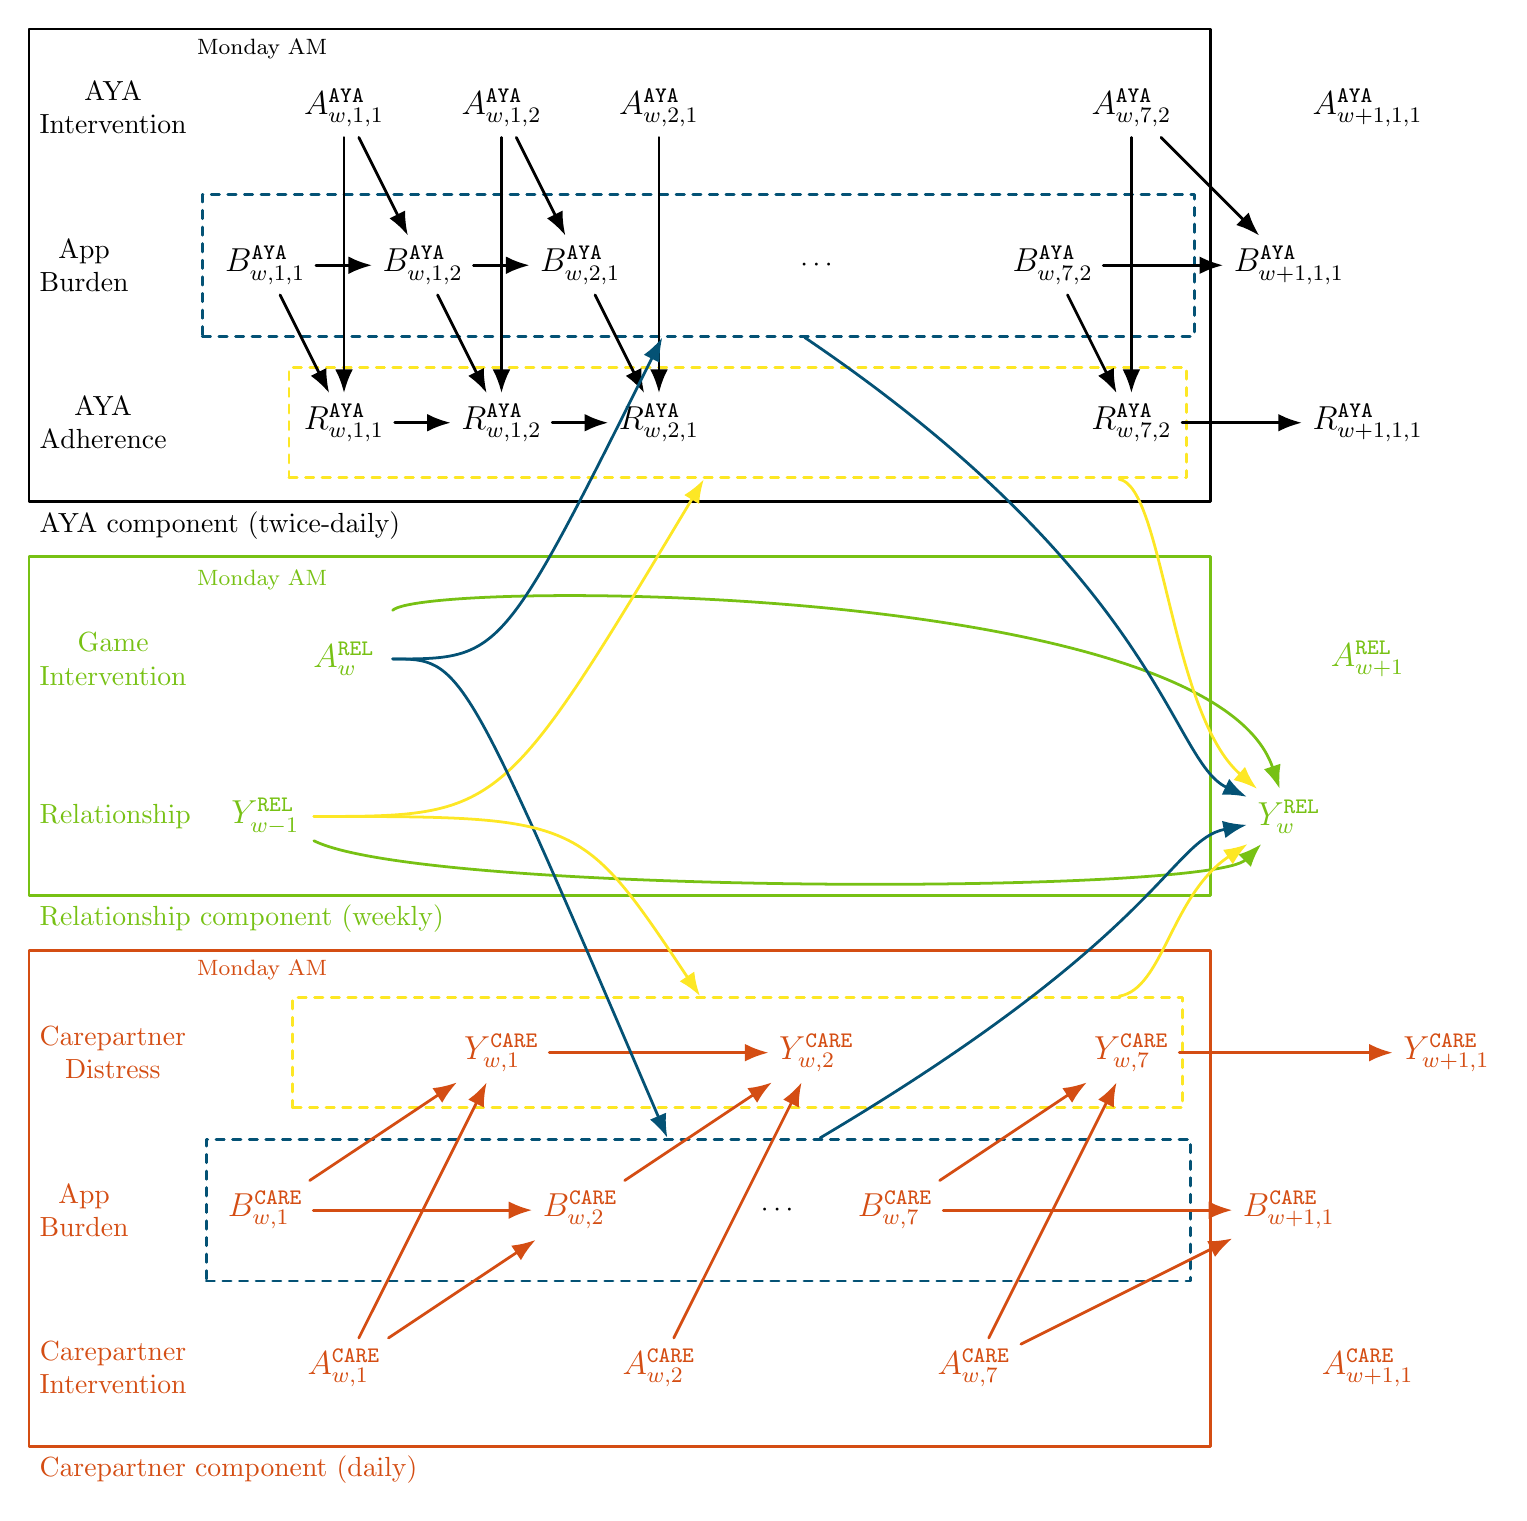
\begin{tikzpicture}[line width=1pt, line cap=round, line join=round]

\def\leftPoint{-3} 
% Carepartner component
\def\btw_color{red}
\def\h{0}; \def\com{C};
\node[right, text=red] at (\leftPoint, -1.3+\h) {Carepartner component (daily)};
  \draw[draw=red] (\leftPoint,-1+\h) rectangle (12,5.3+\h);
  \foreach \z/\hh/\d in {0/0/1, 4/2/2, 8/12/7} {
      \foreach \x/\y/\t/\n in {1/0/A/A, 0/2/U/B, 3/4/S/Y} {
        \node[draw=none, minimum size=0.25cm, text=red] (\t$^{\com}_{t+\hh}$) at (\x + \z, \y + \h) {\large$\n^{\Care}_{w,\d}$};
      }
  }
  \foreach \z/\hh/\d in {14/14/1} {
      \foreach \x/\y/\t/\n in {0/0/A/A, -1/2/U/B, 1/4/S/Y} {
        \node[draw=none, minimum size=0.25cm, text=red] (\t$^{\com}_{t+\hh}$) at (\x + \z, \y + \h) {\large$\n^{\Care}_{w+1,\d}$};
      }
  }
  \node[rectangle, draw, minimum width=12.5cm, minimum height=1.8cm, color = blue, align = right, dashed] (US$^{\com}$) at (5.5, 2+\h){};

  \node[rectangle, draw, minimum width=11.3cm, minimum height=1.4cm, color = viridisYellow, align = right, dashed] (ALLS$^{\com}$) at (6, 4+\h){};
  
  \draw[-{Latex[length=3mm]}, draw=red] (U$^{\com}_{t+0}$)--(U$^{\com}_{t+2}$);
  \draw[-{Latex[length=3mm]}, draw=red] (U$^{\com}_{t+0}$)--(S$^{\com}_{t+0}$);
  \draw[-{Latex[length=3mm]}, draw=red] (S$^{\com}_{t+0}$)--(S$^{\com}_{t+2}$);
  \draw[-{Latex[length=3mm]}, draw=red] (A$^{C}_{t+0}$)--(U$^{C}_{t+2}$);
  \draw[-{Latex[length=3mm]}, draw=red] (A$^{C}_{t+0}$)--(S$^{C}_{t+0}$);

  \draw[-{Latex[length=3mm]}, draw=red] (A$^{C}_{t+2}$)--(S$^{C}_{t+2}$);
  \draw[-{Latex[length=3mm]}, draw=red] (U$^{C}_{t+2}$)--(S$^{C}_{t+2}$);

  \draw[-{Latex[length=3mm]}, draw=red] (U$^{\com}_{t+12}$)--(U$^{\com}_{t+14}$);
  \draw[-{Latex[length=3mm]}, draw=red] (U$^{\com}_{t+12}$)--(S$^{\com}_{t+12}$);
  \draw[-{Latex[length=3mm]}, draw=red] (S$^{\com}_{t+12}$)--(S$^{\com}_{t+14}$);
  \draw[-{Latex[length=3mm]}, draw=red] (A$^{C}_{t+12}$)--(U$^{C}_{t+14}$);
  \draw[-{Latex[length=3mm]}, draw=red] (A$^{C}_{t+12}$)--(S$^{C}_{t+12}$);
  
  \node at (6.5, 2+\h) {$\cdots$};


% Shared component
\def\h{7}; \def\com{E};
\node[right, text=mygreen] at (\leftPoint, -1.3+\h) {Relationship component (weekly)};
  \draw[draw=mygreen] (\leftPoint,-1+\h) rectangle (12,3.3+\h);
  \node[draw=none, minimum size=1.2cm, text=mygreen] (U$^{\com}_{t+0}$) at (0, 0+\h) {\large$Y^{\EDGE}_{w-1}$};
  \node[draw=none, minimum size=1.2cm, text=mygreen] (A$^{\com}_{w(t)}$) at (1, 2 + \h) 
  {\large$A^{\EDGE}_{w}$};
  
  \node[draw=none, minimum size=0.25cm, text=mygreen] (A$^{\com}_{w(t+14)}$) at (14, 2 + \h) 
  {\large$A^{\EDGE}_{w+1}$};
  \node[draw=none, minimum size=0.25cm, text=mygreen] (U$^{\com}_{t+14}$) at (13, 0 + \h) {\large$Y^{\EDGE}_{w}$};

    
% AYA component
\def\h{12}; \def\com{A};
\node[right] at (\leftPoint, -1.3+\h) {AYA component (twice-daily)};
  \draw (\leftPoint,-1+\h) rectangle (12,5+\h);

  \foreach \z/\hh/\d/\k in {0/0/1/1, 2/1/1/2, 4/2/2/1, 10/13/7/2} {
      \foreach \x/\y/\t/\n in {1/0/S/R, 0/2/U/B, 1/4/A/A} {
        \node[draw=none, minimum size=0.25cm] (\t$^{\com}_{t+\hh}$) at (\x + \z, \y + \h) {\large$\n^{\AYA}_{w, \d, \k}$};
      }
  }
  \foreach \z/\hh/\d/\k in {13/14/1/1} {
      \foreach \x/\y/\t/\n in {1/0/S/R, 0/2/U/B, 1/4/A/A} {
        \node[draw=none, minimum size=0.25cm] (\t$^{\com}_{t+\hh}$) at (\x + \z, \y + \h) {\large$\n^{\AYA}_{w+1, \d, \k}$};
      }
  }

    \node[rectangle, draw, minimum width=12.6cm, minimum height=1.8cm, color = blue, align = right, dashed] (US$^{\com}$) at (5.5, 2+\h){};

    \node[rectangle, draw, minimum width=11.4cm, minimum height=1.4cm, color = viridisYellow, align = right, dashed] (ALLS$^{\com}$) at (6, 0+\h){};


  \draw[-{Latex[length=3mm]}, color = black] (A$^{\com}_{t+0}$)--(S$^{\com}_{t+0}$);
  \draw[-{Latex[length=3mm]}, color = black] (A$^{\com}_{t+0}$)--(U$^{\com}_{t+1}$);
  \draw[-{Latex[length=3mm]}, color = black] (S$^{\com}_{t+0}$)--
  (S$^{\com}_{t+1}$);
  \draw[-{Latex[length=3mm]}, color = black] (U$^{\com}_{t+0}$)--(S$^{\com}_{t+0}$);
  \draw[-{Latex[length=3mm]}, color = black] (U$^{\com}_{t+0}$)--(U$^{\com}_{t+1}$);

    \draw[-{Latex[length=3mm]}, color = black] (A$^{\com}_{t+1}$)--(S$^{\com}_{t+1}$);
  \draw[-{Latex[length=3mm]}, color = black] (A$^{\com}_{t+1}$)--(U$^{\com}_{t+2}$);
  \draw[-{Latex[length=3mm]}, color = black] (S$^{\com}_{t+1}$)--(S$^{\com}_{t+2}$);
  \draw[-{Latex[length=3mm]}, color = black] (U$^{\com}_{t+1}$)--(S$^{\com}_{t+1}$);
  \draw[-{Latex[length=3mm]}, color = black] (U$^{\com}_{t+1}$)--(U$^{\com}_{t+2}$);

      \draw[-{Latex[length=3mm]}, color = black] (A$^{\com}_{t+2}$)--(S$^{\com}_{t+2}$);
      \draw[-{Latex[length=3mm]}, color = black] (U$^{\com}_{t+2}$)--(S$^{\com}_{t+2}$);

      \draw[-{Latex[length=3mm]}, color = black] (A$^{\com}_{t+13}$)--(S$^{\com}_{t+13}$);
  \draw[-{Latex[length=3mm]}, color = black] (A$^{\com}_{t+13}$)--(U$^{\com}_{t+14}$);
  \draw[-{Latex[length=3mm]}, color = black] (S$^{\com}_{t+13}$)--(S$^{\com}_{t+14}$);
  \draw[-{Latex[length=3mm]}, color = black] (U$^{\com}_{t+13}$)--(S$^{\com}_{t+13}$);
  \draw[-{Latex[length=3mm]}, color = black] (U$^{\com}_{t+13}$)--(U$^{\com}_{t+14}$);

    \node at (7, 2+\h) {$\cdots$};

% all variable labels
% AYA

\node[right, color = black, align = center] at (\leftPoint + 2, 4.75+12) {\footnotesize{Monday AM}};

\node[right, color = mygreen, align = center] at (\leftPoint + 2, 5+5) {\footnotesize{Monday AM}};

\node[right, color = red, align = center] at (\leftPoint + 2, 5.05) {\footnotesize{Monday AM}};

\node[right, color = black, align = center, text=black] at (\leftPoint, 4+12) {AYA \\ Intervention};
\node[right, color = black, align = center, text=black] at (\leftPoint, 2+12) {App \\ Burden};
\node[right, color = black, align = center, text=black] at (\leftPoint, 0+12) {AYA\\ Adherence};

% Shared
\node[right, color = black, align = center, text=mygreen] at (\leftPoint, 0+7) {Relationship};
\node[right, color = black, align = center, text=mygreen] at (\leftPoint, 2+7) {Game \\ Intervention};
% \node[right, color = black, align = center] at (\leftPoint, 4+7) {Weekly \\ Observation};

% Carepartner
\node[right, color = black, align = center, text=red] at (\leftPoint, 4) {Carepartner \\ Distress};
\node[right, color = black, align = center, text=red] at (\leftPoint, 2) {App \\ Burden};
\node[right, color = black, align = center, text=red] at (\leftPoint, 0) {Carepartner \\ Intervention};


% week label
% \node[right, color = viridisCyan] at (\leftPoint-0.5, 5.5+\h) {Week $w$};
% \draw[color = viridisCyan, dashed] (\leftPoint-0.5,-1.7) rectangle (12.5,17.2);
% \node[right, color = viridisCyan] at (13, 5.5+\h) {Week $w+1$};

\draw[-{Latex[length=3mm]}, color = mygreen](A$^{E}_{w(t)}$).. controls (2,10) and (12,10) .. (U$^{E}_{t+14}$);

\draw[-{Latex[length=3mm]}, color = mygreen](U$^{E}_{t+0}$).. controls (2,6) and (12,6) ..(U$^{E}_{t+14}$);

\draw[-{Latex[length=3mm]}, color = blue](US$^{A}$) .. controls (11.4,10) and (11.5,7.7) ..(U$^{E}_{t+14}$);

% \node[color = viridisCyan] at (13, 8) {(+)};

\draw[-{Latex[length=3mm]}, color = blue](US$^{C}$).. controls (11.4,5.5) and (11.5,6.7) ..(U$^{E}_{t+14}$);

\draw[-{Latex[length=3mm]}, color = viridisYellow](ALLS$^{A}$) .. controls (11.4,11.2) and (11.5,8.3) ..(U$^{E}_{t+14}$);

% \node[color = viridisCyan] at (13, 8) {(+)};

\draw[-{Latex[length=3mm]}, color = viridisYellow](ALLS$^{C}$).. controls (11.4,4.8) and (11.5,6) ..(U$^{E}_{t+14}$);


% weekly relationship to AYA component
\draw[-{Latex[length=3mm]}, color = blue](A$^{E}_{w(t)}$).. controls (3,9) ..(US$^{A}$);

\draw[-{Latex[length=3mm]}, color = viridisYellow](U$^{E}_{t+0}$).. controls (3,7) ..(ALLS$^{A}$);

\draw[-{Latex[length=3mm]}, color = blue](A$^{E}_{w(t)}$).. controls (2.5,9) ..(US$^{C}$);


\draw[-{Latex[length=3mm]}, color = viridisYellow](U$^{E}_{t+0}$).. controls (4,7) ..(ALLS$^{C}$);

% \draw[dashed][-{Latex[length=3mm]}, color = gray](S$^{A}_{t+0}$) .. controls (3,10) .. (S$^{C}_{t+2}$);
% \draw[dashed][-{Latex[length=3mm]}, color = gray](S$^{A}_{t+1}$) .. controls (3,10) .. (S$^{C}_{t+2}$);

% \draw[dashed][-{Latex[length=3mm]}, color = gray](S$^{C}_{t+0}$) .. controls (3,5) .. (S$^{A}_{t+2}$);

% \draw[-{Latex[length=3mm]}, color = gray](S$^{C}_{t+0}$) .. controls (1,10) .. (S$^{A}_{t+1}$);
% \draw[-{Latex[length=3mm]}, color = gray](S$^{C}_{t+0}$) .. controls (1,10) .. (S$^{A}_{t+2}$);
\end{tikzpicture}

%     \caption{Simplified ADAPTS-HCT causal DAG for week $w$. Arrows between nodes indicate direct causal effects. An arrow to a dashed block is equivalent to having an arrow to each of the nodes within the block. Context variables are omitted. Arrows into all three actions are omitted.}
%     \label{fig:DAG2}
% \end{wrapfigure}

\end{document}